\documentclass[aspectratio=169]{beamer}

% Text in English
\usepackage[english]{babel}

% Document metadata
\title{Classical and Quantum Computing techniques for Dihedral error correcting codes}
\subtitle{Beamer template}
\author[TL]{Abdul Fatah, Ian Mcloughlin}
\institute{ATU - Atlantic Technological University, Galway}
\date{\today}

% Image for the title page (use the includegraphics option to size/position it correctly)
\titlegraphic{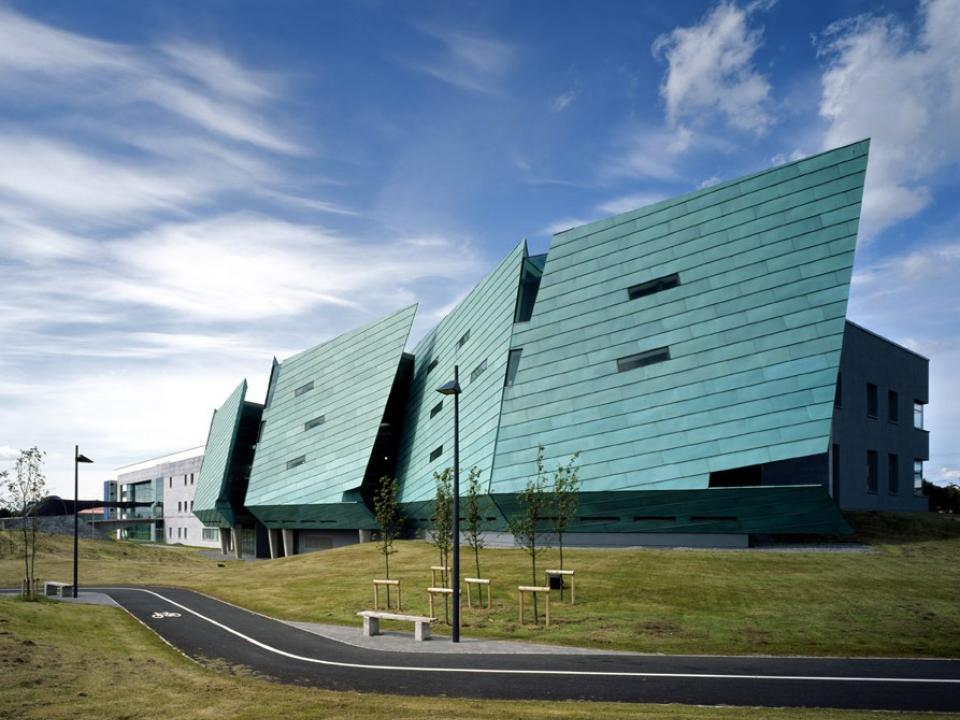
\includegraphics[height=\paperheight]{images/ATUgalway.jpg}}

\usetheme[sectionstyle=style2]{trigon}

% Define the logos to use (comment if there is no logo)
\biglogo{atulogo31.jpg} % Used only on the cover
\biglogo{}
\smalllogo{atulogo1.png} % Used in the upper right corner of normal frames

% ------ If you want to change the default theme colors, do it here ------
\definecolor{tPrim}{HTML}{EA7600}   % 716
\definecolor{tSec}{HTML}{B1B1B1}    % cool gray
\definecolor{tAccent}{HTML}{002F6C} % 294

 
%------ Packages and definitions used for this demo. Can be deleted ------
\usepackage{appendixnumberbeamer} % To use \appendix command
\pdfstringdefDisableCommands{% Fix hyperref translate warning with \appendix
\def\translate#1{#1}%
}
\usepackage{graphicx}
\usepackage[export]{adjustbox}
\usepackage{pgf-pie} % For pie charts 
\usepackage{caption} % For subfigures
\usepackage{subcaption} % For subfigures
\usepackage{xspace}
\newcommand{\themename}{\textbf{\textsc{USACHtheme}}\xspace}
\usepackage[scale=2]{ccicons} % Icons for CC-BY-SA
\usepackage{booktabs} % Better tables


%==============================================================================
%                               COMENZAR DOCUMENTO
%==============================================================================
\begin{document}

%--------------------------------------
% Create title frame
\titleframe

%--------------------------------------
% Table of contents
\begin{frame}{Overview}
  \setbeamertemplate{section in current}[sections numbered]
  \tableofcontents[hideallsubsections]
\end{frame}


%==============================================
\section{Introduction}
%==============================================
\begin{frame}{\insertsectionhead}
  \framesubtitle{ Quantum Computing and Quantum Information Science}
  
  \hline Quantum Computing and Quantum Information Science have the potential to disrupt, not just the Information and Communications Technology sector, but our understanding of the physical world.\\


    \begin{figure}
    %\centering
    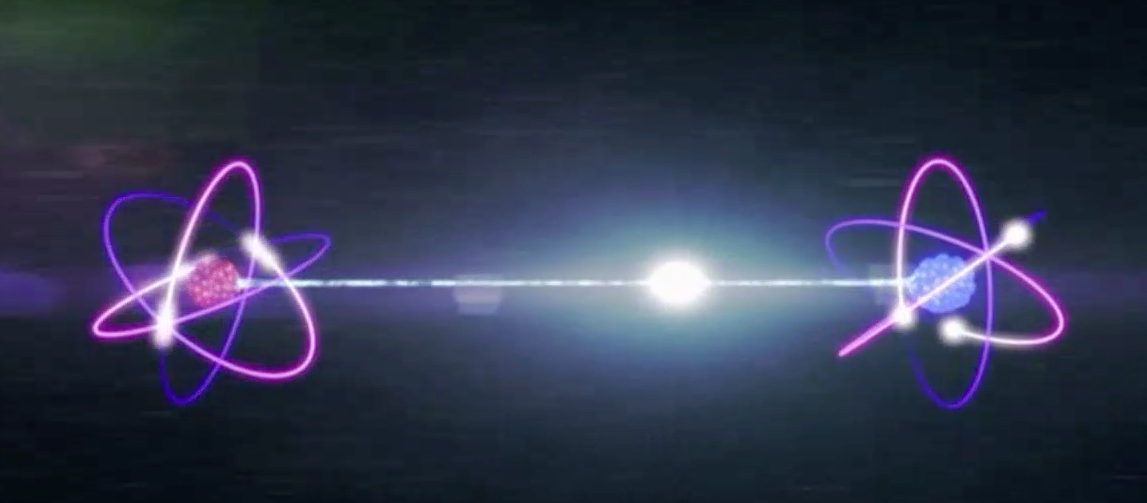
\includegraphics[width=0.5\linewidth, height=4cm]{images/Qentangled.png}
    \caption{Quantum Characteristics}
    %\label{fig:my_label}
    \end{figure}
%\begin{subfigure}{0.5\textwidth}
%\includegraphics[width=0.9\linewidth, height=6cm]{overleaf-logo} 
%\caption{Caption1}
%\label{fig:subim1}
%\end{subfigure}
%\begin{subfigure}{0.5\textwidth}
%\includegraphics[width=0.9\linewidth, height=6cm]{mesh}
%\caption{Caption 2}
%\label{fig:subim2}
%\end{subfigure}

%\caption{Caption for this figure with two images}
%\label{fig:image2}
\end{figure}
  
  \end{frame}
  
  \begin{frame}
  \themename is a modern, elegant and versatile theme for Beamer, based on the TRIGON theme.
  \vfill
  \themename comes with a lot of interesting extra features
  \begin{itemize}
    \item Multiple style variations for title, section, and regular slides
    \item Easy customization of theme colors
    \item Lots of handy options for tweaking the layout
  \end{itemize}
\end{frame}


%==============================================
\section{Layout}
%==============================================

\subsection{Variaciones de diseño}

\begin{frame}[fragile=singleslide]{\insertsectionhead}
  \framesubtitle{\insertsubsectionhead}
  El estilo general para el título, la sección y los marcos regulares puede cambiarse fácilmente con opciones sencillas. Estos son algunos ejemplos para la página del título
  \begin{figure}[ht!]
    \begin{subfigure}[b]{0.3\textwidth}
      \frame{\includegraphics[width=\textwidth]{screenshots/layout_example-03.jpg}}
      \caption*{plain}
    \end{subfigure}
    \hspace{\fill}
    \begin{subfigure}[b]{0.3\textwidth}
      \frame{\includegraphics[width=\textwidth]{screenshots/layout_example-02.jpg}}
      \caption*{style1}
    \end{subfigure}
    \hspace{\fill}
    \begin{subfigure}[b]{0.3\textwidth}
      \frame{\includegraphics[width=\textwidth]{screenshots/layout_example-01.jpg}}
      \caption*{style2 (default)}
    \end{subfigure}
  \end{figure}
\end{frame}

%--------------------------------------
\subsection{Fuentes}

\begin{frame}
  \frametitle{\insertsectionhead}
  \framesubtitle{\insertsubsectionhead}
  Este tema utiliza \textit{Source Sans Pro} para todos los elementos por defecto. Esto se puede desactivar mediante la opción  \texttt{usesourcefonts=false}.
  \vfill
  Se puede añadir énfasis utilizando \textbf{bold} typeface, \textit{italic},
  \alert{alert} o {\color{tPrim}{simple colors}}.
  \vfill
   Las ecuaciones también se tipifican con esta fuente
  \begin{equation*}
    F(x|\mu,s) = \int_{-\infty}^x s^{-1}\left(1+e^{-\frac{v-\mu}{s}}\right)^{-2} e^{-\frac{v-\mu}{s}}\;\mathsf{d}v = \frac{1}{1+e^{-\frac{x-\mu}{s}}}
  \end{equation*}
\end{frame}


%==============================================
\section{Elements}
%==============================================
\subsection{Graphics}
\begin{frame}{\insertsectionhead}
  \framesubtitle{\insertsubsectionhead}
  \begin{columns}[c, onlytextwidth]
    \column{0.47\textwidth}
    Use the theme color \texttt{tPrim}, \texttt{tSec}, \texttt{tGrey} y
    \texttt{tAccent} para que los gráficos se ajusten directamente al tema principal de la presentación.
    \vfill
    \begin{itemize}
      \item simple variants with \texttt{color!x} to lighten or darken colors
    \end{itemize}
    \hfill
    \column{0.47\textwidth}
    \center
    \resizebox{0.9\textwidth}{!}{%
      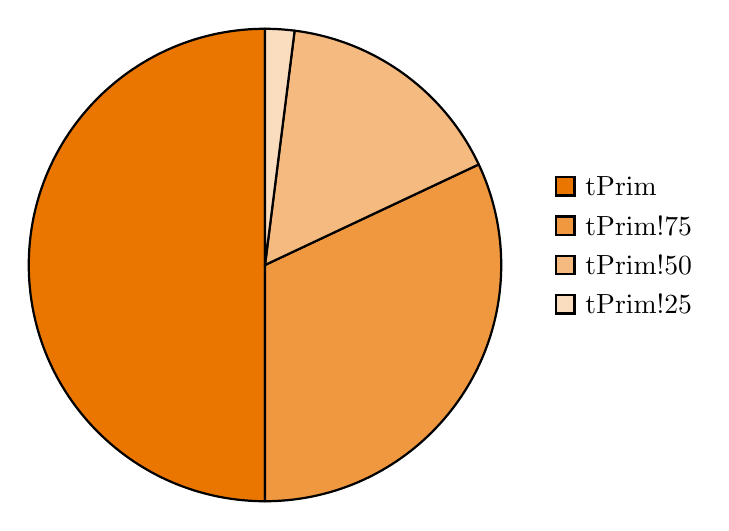
\begin{tikzpicture}
        \pie[color={tPrim, tPrim!75, tPrim!50, tPrim!25},
        rotate=90, hide number, text= legend]
        {50/tPrim, 32/tPrim!75, 16/tPrim!50, 2/tPrim!25}
      \end{tikzpicture}
    }
  \end{columns}
\end{frame}

\subsection{lists}
\begin{frame}{\insertsectionhead}
  \framesubtitle{\insertsubsectionhead}
  \begin{columns}[T,onlytextwidth]
    \column{0.28\textwidth}
    Items
    \begin{itemize}
      \item Item 1
        \begin{itemize}
          \item Subitem 1
          \item Subitem 2
        \end{itemize}
      \item Item 2
      \item Item 3
    \end{itemize}

    \column{0.42\textwidth}
    enumerations
    \begin{enumerate}
      \item The Fellowship of the Ring,
      \item The Two Towers,
      \item The Return of the King.
    \end{enumerate}

    \column{0.30\textwidth}
    Descriptions
    \begin{description}
      \item[Trigon] Modern. \item[Default] Outdated.
    \end{description}
  \end{columns}
\end{frame}

%--------------------------------------
\subsection{Figure}
\begin{frame}
  \frametitle{\insertsectionhead}
  \framesubtitle{\insertsubsectionhead}

  \begin{figure}
    \newcounter{density}
    \setcounter{density}{20}
    \begin{tikzpicture}
      \def\couleur{tAccent}
      \def\color{tSec}
      \path[coordinate] (0,0)  coordinate(A)
        ++( 60:5cm) coordinate(B)
        ++(-60:5cm) coordinate(C);
      \path[coordinate] (0,0)  coordinate(D)
        ++(60:5cm) coordinate(E)
        ++(180:5cm) coordinate(F);
      \draw[fill=\color!\thedensity] (A) -- (B) -- (C) -- cycle;
      \draw[fill=\color!\thedensity] (D) -- (E) -- (F) -- cycle;
      \foreach \x in {1,...,15}{%
        \pgfmathsetcounter{density}{\thedensity+10}
        \setcounter{density}{\thedensity}
        \path[coordinate] coordinate(X) at (A){};
        \path[coordinate] (A) -- (B) coordinate[pos=.15](A)
          -- (C) coordinate[pos=.15](B)
          -- (X) coordinate[pos=.15](C);
        \draw[fill=\color!\thedensity] (A)--(B)--(C)--cycle;
      }
      \setcounter{density}{20}
      \foreach \x in {1,...,15}{%
        \pgfmathsetcounter{density}{\thedensity+10}
        \setcounter{density}{\thedensity}
        \path[coordinate] coordinate(X) at (D){};
        \path[coordinate] (D) -- (E) coordinate[pos=.15](D)
          -- (F) coordinate[pos=.15](E)
          -- (X) coordinate[pos=.15](F);
        \draw[fill=\color!\thedensity] (D)--(E)--(F)--cycle;
      }
    \end{tikzpicture}
    \caption{Triángulos rotados desde
    \href{http://www.texample.net/tikz/examples/rotated-triangle/}{texample.net}.}
  \end{figure}
\end{frame}

%--------------------------------------
\subsection{Table}
\begin{frame}
  \frametitle{\insertsectionhead}
  \framesubtitle{\insertsubsectionhead}
  \begin{table}[H]
    \centering
    \caption{tabla ejemplo}
    \begin{tabular}{@{} lccc @{}}
      \toprule
      & \textbf{Velocity} & \textbf{Angle}  & \textbf{Vertical force} \\
      & $U$ & $\alpha$  & $F_z$ \\
      & [m/s] & [$^\circ$]  & [N] \\
      \midrule
      2D simulation  & 9 & 2 & 9.23 \\
      3D simulation  & 10.0 & 3 & 15.039 \\
      Experiment A   & 11.31 & 2.5 & 13.2 \\
      Experiment B   & 11.26 & 2.7 & 12.6 \\
      Experiment C   & 11.33 & 2.47 & 13.6 \\
      \bottomrule
    \end{tabular}
  \end{table}

\end{frame}

%--------------------------------------
\subsection{blocks}
\begin{frame}
  \frametitle{\insertsectionhead}
  \framesubtitle{\insertsubsectionhead}
  \begin{block}{Regular block}
    Un bloque normal
  \end{block}
  \begin{alertblock}{Alert block}
    Something important
  \end{alertblock}
  \begin{exampleblock}{Example block}
    No difference to regular blocking to prevent excessive distraction
  \end{exampleblock}
\end{frame}

%--------------------------------------
\subsection{Frame Footer}
{
\setbeamertemplate{frame footer}{footer}
\begin{frame}[fragile]
  \frametitle{\insertsectionhead}
  \framesubtitle{\insertsubsectionhead}
    \themename defines a custom template to add a text to the footer. It can be set via
    \begin{verbatim}\setbeamertemplate{frame footer}{My custom footer}\end{verbatim}
\end{frame}
}

\begin{frame}{References}
  Algunas referencias para mostrar [allowframebreaks] \cite{knuth92,ConcreteMath,Simpson,Er01,greenwade93}
\end{frame}

%==============================================
\section{Conclusion}
%==============================================
\begin{frame}{Resume}

  Get this theme's source and demo presentation at

  \begin{center}\url{gitlab.com/thlamb/beamertheme-trigon}\end{center}

  As for \textsc{metropolis}, \themename is licensed under a
  \href{http://creativecommons.org/licenses/by-sa/4.0/}{Creative Commons
  Attribution-ShareAlike 4.0 International License}.

  \begin{center}\ccbysa\end{center}

\end{frame}

%==============================================
%\begin{frame}[standout]
%  Questions?
%\end{frame}

\appendix

\begin{frame}[fragile]{backup slides}
  Sometimes it's helpful to add slides to the end of your presentation to refer to during questions from the audience.

  The best way to do this is to include the\verb|appendixnumberbeamer|
  in your preamble and call \verb|\appendix| before the backing slides.

  \themename will automatically disable slide numbering and progress bars for slides in the appendix.
\end{frame}

\begin{frame}[allowframebreaks]{References}

  \bibliography{demo}
  \bibliographystyle{abbrv}

\end{frame}


\end{document}
